% Use only LaTeX2e, calling the article.cls class and 12-point type.

\documentclass[11pt]{article}

\usepackage[round,semicolon]{natbib}
\usepackage{etoolbox}
\AtBeginEnvironment{quote}{\singlespacing\tiny}
% Use times if you have the font installed; otherwise, comment out the
% following line.

% added by SKH
%\usepackage{lineno}
%\linenumbers

\usepackage{times}
\usepackage{amssymb}
\usepackage{amsmath}

\usepackage[export]{adjustbox}

\usepackage{graphicx}
\graphicspath{ {images/} }

% for adjustwidth
\usepackage{changepage}

% The following parameters seem to provide a reasonable page setup.

\topmargin 0.0cm
\oddsidemargin 0.2cm
\textwidth 16cm 
\textheight 21cm
\footskip 1.0cm

\usepackage{newfloat}
\usepackage{amsmath}
\usepackage[labelfont=bf]{caption}
\usepackage{nameref}
\usepackage{rotating}
\usepackage{color}
\usepackage{float}
\renewcommand{\figurename}{{}}
\renewcommand{\thefigure}{{Figure \arabic{figure}}}

\renewcommand{\tablename}{{}}
\renewcommand{\thetable}{{Table \arabic{table}}}

\newfloat{suppfile}{thp}{losuppfile}
\renewcommand{\thesuppfile}{Supplementary file \arabic{suppfile}}
\floatname{suppfile}{}

\newfloat{suppfig}{thp}{losuppfig}
\renewcommand{\thesuppfig}{Supplementary figure \arabic{suppfig}}
\floatname{suppfig}{}

%
\newfloat{supptable}{thp}{losupptable}
\renewcommand{\thesupptable}{Supplementary table \arabic{supptable}}
\floatname{supptable}{}
%

\renewcommand{\theequation}{Equation \arabic{equation}}

\newcommand{\mutDNA}{\textbf{mutDNA}}
\newcommand{\mutvirus}{\textbf{mutvirus}}
\newcommand{\DNA}{\textbf{DNA}}
\newcommand{\virus}{\textbf{virus}}

\newcommand\skhcomment[1]{{\color{magenta}#1}}
\newcommand\jdbcomment[1]{{\color{red}#1}}


\usepackage{hyperref}
\hypersetup{colorlinks,citecolor=blue,linkcolor=blue,urlcolor=blue}
\hypersetup{colorlinks,citecolor=blue,linkcolor=blue,urlcolor=blue}

\usepackage{seqsplit}

\usepackage{array}
\newcolumntype{P}[1]{>{\raggedright\arraybackslash}p{#1}}

\title{Experimentally Informed Site-Specific Substitution Models Substantially Deepen Viral Divergence Estimates} 

\author
{Sarah K. Hilton$^{1,2}$  and Jesse D. Bloom$^{1,2,}$\\
\\
\normalsize{$^1$Division of Basic Sciences and Computational Biology Program,}\\
\normalsize{Fred Hutchinson Cancer Research Center, Seattle, WA 98109, USA}\\
\normalsize{$^2$Department of Genome Sciences, University of Washington, Seattle, WA}\\
\normalsize{E-mail:  jbloom@fredhutch.org.}\\
}


% Include the date command, but leave its argument blank.

\date{}

\usepackage{setspace}
\onehalfspacing


\begin{document} 

% Make the title.

\maketitle 


\begin{abstract}
\textit{$\leq$ 250 words}   

Molecular dating techniques is often used to estimate the divergence time of many viruses. 
However, these estimates are substantially younger than estimates from methods which do not rely on viral phylogenies. 
This discrepancy is thought to be caused in part by inadequate modeling of purifying selection leading to branch length underestimation. 
Here, we show that substitution models informed by empirical measurements of mutational model constraint better than traditional models and extend branch lengths. 
We used models informed by deep mutational scanning experiments performed in two, highly diverged influenza virus hemagglutinin homologs to optimize the branch lengths of a phylogenetic tree. 
For each experimentally informed model, we observed extension in branch length from the experiment's focal sequence. 
This extension in branch length due to explicit modeling of site-specific purifying selection is observed in the presence and absence of standard methods for modeling site-to-site variation. 
Overall, this study underscores the importance of modeling purifying selection when estimating branch lengths and, by extension, divergence dates. 
\skhcomment{from JDB: also shows a way to actually do this in addition to showing importance.}

\end{abstract}

\clearpage

\section*{Introduction} 
\skhcomment{from JDB: what is the "age" of a virus? Maybe "divergence time of viral lineages"}
skhcomment{from JDB: what is the less than a million actually? "Old" is not the right phrase.}
Estimating the divergence time of viral lineages of a virus is essential to understanding its evolutionary history, including its emergence, spread, and past zoonoses. 
This estimation is commonly done using the concept a ``molecular clock" to transform the branch lengths of the viral phylogenetic tree into age in years. 
However, this molecular dating technique often underestimates the age of many viruses, including measles, foamy virus, and ebola \skhcomment{(citations)}, compared to other methods which are independent of the viral phylogeny. 
For example, SIV (the original source of HIV) is estimated to be less than a million years old based on the viral phylogeny \citep{sharp2000origins,wertheim2009dating,worobey2010island} but estimated to be several million years old based on the host tree or endogenous retroviral elements  \citep{compton2013host} \skhcomment{(other citations)}. 
Overall, there is a systematic and substantially large underestimation of of branch length on viral phylogenies. 
\skhcomment{long branches}

Branch length underestimation is due, in part, to strong purifying selection masking the evolutionary signal in the observed sequences. 
Purifying selection can lead to mutational saturation, where multiple unobserved, substitutions occur at a single site along a long branch and erase the divergence signal \citep{holmes2003molecular}.
Furthermore, proteins do not have equal preference for all amino acids at all sites, this evident by a simple visual inspection of a multiple sequence alignment. 
How many and which amino acids tolerated at each site of the protein generate a site-specific expected rate of change. 
Failing to account for these site-specific constraints will lead to branch length underestimation. 
\skhcomment{you will have mutational saturation no matter what - this is a separate, addressable issue?}
\skhcomment{talk about the high mutation rate in viruses?}

Substitution models that incorportate site-to-site rate variation have been developed to decrease the bias in long branch estimation. 
The most common strategy is to allow a single rate-controlling parameter to vary according to some statistical distribution, such as a $\Gamma$-distributed $\omega$ (~dN/dS) \citep{yang2000codon}. 
This flexibility in the value of $\omega$ accounts for the site-to-site rate variation by allow some sites to have a higher dN/dS value than others. 
While this modification is simple and only requires the addition of one extra parameter, it does not describe site-specificity in its stationary state. 
That is, at evolutionary equilibrium, this model still assumes that each site in the protein evolves identically.  

An alternative approach is to model the site-specific amino-acid frequencies explicitly, such as those models in the mutation-selection family \citep{halpern1998evolutionary}. 
In these models, each amino-acid at each site in the protein is described by its own parameter and these differences are reflected in the stationary state of the model. 
The rate of change at a given site is controlled by these amino acid profiles and can now vary from site to site, as expected based on observations in nature. 
Importantly, these rate variations are not constrained to an arbitrary statistical distribution but by parameters with a direct biological interpretation. 

Mutation-selection models are presumably more biologically relevant but pose more practical challenges than the $\Gamma\omega$ models. 
These models are highly parametrized with 19 free parameters (the 20 amino acid preferences are constrained to sum to one) per site leading to thousands of parameters for the length of a normal protein. 
One way to avoid overfitting is to implement the model as a mixture model in either a bayesian \citep{lartillot2004bayesian} or maximum likelihood framework \citep{si2008empirical}. 

Alternatively, you can reduce the parameter space by defining the amino-acid frequencies \textit{a priori}. 
We have shown previously that we can define an Experimentally Informed Codon Model (ExpCM) \citep{bloom2014experimentally,bloom2014informed} from the mutation-selection family using measurements from deep mutational scanning \citep{fowler2014deep}, a high-throughput functional assay. 
ExpCM are therefore defined by amino-acid preferences measured in a \textit{single} genetic background and do not reflect any epistatic changes which may have occurred over the virus's evolutionary history. 
But they contain no more parameters than the traditional codon models while maintaining a site-specific stationary state. 
We hypothesize that the ExpCM will estimate longer branches than the traditional models due to the protein-specific description of purifying selection. 
\skhcomment{CAT model has been shown to work well (better) on saturated data.}

In order to test this hypothesis, we compared the branch lengths of a influenza virus HA phylogenetic trees optimized by different substitution models. 
We found that the ExpCM did extend the length of branches from the focal sequence on the tree \skhcomment{define focal} and that this extension was seen even in the context of $\Gamma$-distributed rate variation. 
Furthermore, we found this extension occurred even in the presence of $\Gamma$-distributed $\omega$, indicating that they are both important for modeling purifying selection. 
This supports the conclusion that modeling purifying selection, especially in a model with a non-uniform stationary state, is important to estimating the branch lengths on phylogenetic trees. 

\section*{Results and Discussion}

\subsection*{Substitution models}

\begin{figure}[H]
\centerline{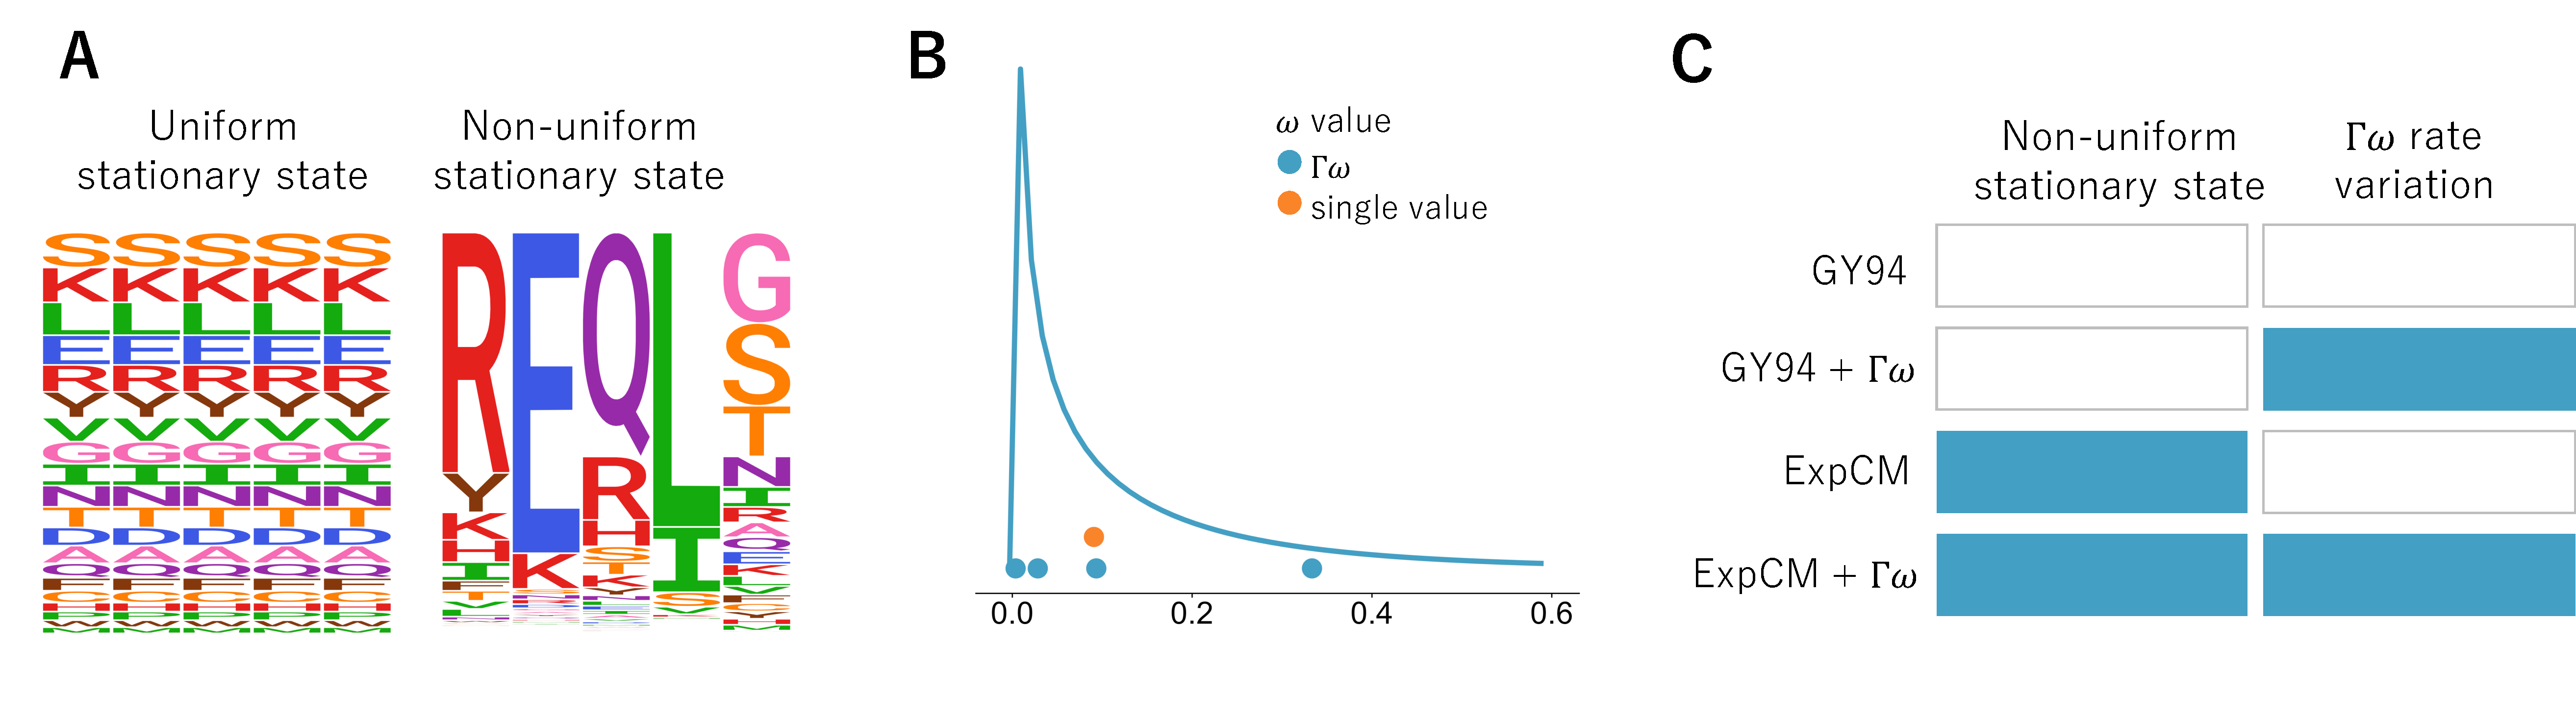
\includegraphics[width=0.55\textwidth]{figures/model_feature.pdf}}
\caption{\label{fig:model_feature}
\textbf{Comparison of substitution model features.}
\jdbcomment{This figure is too big. Maybe put the three panels side-by-side, increase the space between panels, and increase the font sizes. The logo stacks are kind of tall relative to their width.}
Site-specific amino-acid profiles and $\Gamma$-distributed rate variation are both substitution model features which have been shown or theorized to lengthen branches. 
The models YNGKP M0, YNGKP M5, ExpCM, and ExpCM+$\Gamma\omega$ represent all possible combinations of these two features. 
Blue indicates presence and white indicates absence of a feature. 
from \ref{tab:wsn_low_params}
}
\end{figure}

\skhcomment{opening sentence or two about modeling site-to-site rate variation and/or purifying selection}

Codon substitution models commonly include a parameter ($\omega$) which describes the relative rate of non-synonymous to synonymous change to account for purifying selection or site-to-site rate variation more generally. 
This parameter can be constrained to one value, representing a gene-wide average rate, or allowed to vary among sites following some statistical distribution, commonly a $\Gamma$-distribution (\ref{fig:model_feature}B). 
By allowing $\omega$ to vary among the sites, this models acknowledges that some sites evolve faster or slower than others. 
However, in practical implementation the distribution is discretized into some number of categories (commonly four) and $\omega$ takes on the mean of each category. 

Another strategy to account for purifying selection and site-to-site rate variation is to use a model with a non-uniform stationary state (\ref{fig:model_feature}A). 
In this framework, differences in rate between sites is modeled explicitly by site-specific amino-acid frequency parameters. 
These parameters describe the ''preference" for a given amino acid at a given site. 
According to this model, the rate of change at a "constrained" site, which prefers very few amino acids, is much slower than the rate of change at a tolerant site, which prefers many amino acids equally. 

The challenge of a model with a non-uniform stationary state is that all 19 * L (sites in the protein) amino acid preference parameters have to be defined. 
In this study, we chose to use non-uniform stationary state model called ExpCM which defines these parameters using the measurements from a high-throughput functional assay called Deep Mutational Scanning (DMS). 
DMS measures the effect of every single amino acid change on some aspect of protein function. 
We used two deep mutational scans of influenza virus surface protein hemagglutinin (HA) which measured the effect of mutations on viral growth. 

The models we chose to use in this study represent all four combinations of these two features (\ref{fig:model_feature}C). 
The GY94 model has a uniform stationary state while the ExpCM has a non-uniform stationary state and each model can be implemented with a $\Gamma$-distributed $\omega$. 
Therefore, we can example the effect of one feature (stationary state or $\Gamma\omega$) while controlling for the presence of the other feature. 

\subsection*{Effect of stationary state and rate variation on branch length estimation}

\begin{figure}[H]
\centerline{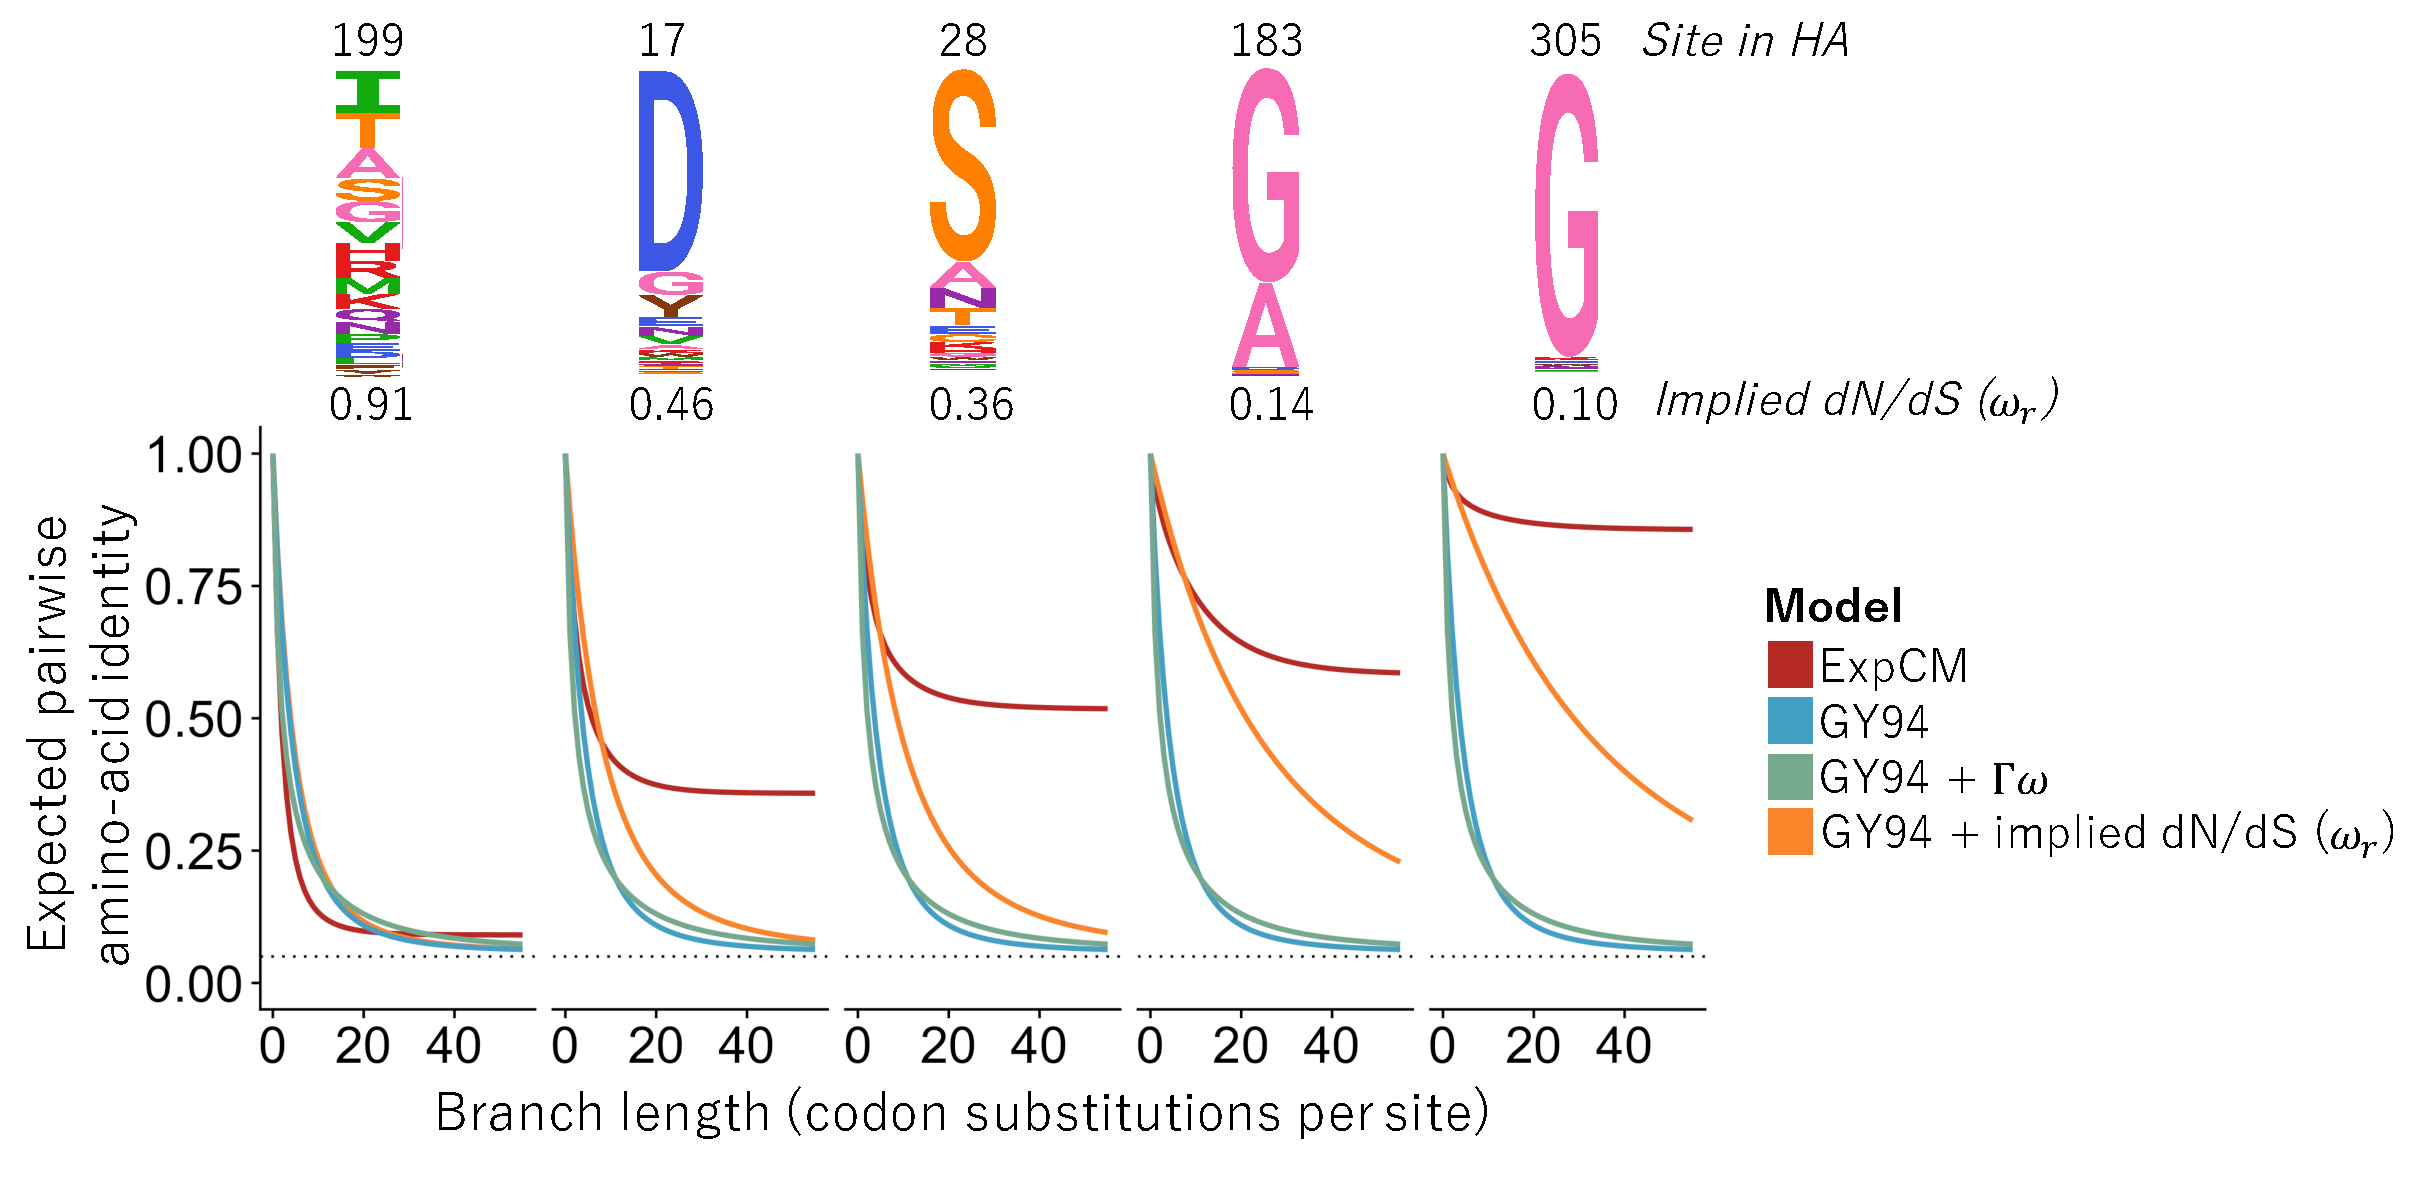
\includegraphics[width=0.75\textwidth]{figures/decay.pdf}}
\caption{\label{fig:decay}
\jdbcomment{I still think text could be bigger. Logo stacks still show trimming, maybe a bit tall? The Model key could probably be to the right or left.}
\textbf{Effect of stationary state and rate variation on long branch estimation.}
The expected pairwise identity trajectories were calculated using \ref{eq:f} and models described in \ref{tab:wsn_low_params}.
The trajectories of the YNKGP M0 (blue) and YNGKP M5 (green) do not vary from panel to panel because neither model is site-specific. 
The deviation in trajectory of the ExpCM (red) from the YNGKP M0 (blue) increases from left to right as the mutational constraint of the amino-acid profile increases (logoplots, above). 
The deviation in trajectory of the YNGKP model with a site-specific $\omega$ value inferred from the ExpCM (yellow, \ref{eq:w_r}) is also positively correlated with the constraint of the site-specific amino-acid profiles but the effect size is smaller. 
}
\end{figure}

To explore the effect of substitution model choice on branch length estimation, we first examined how the relationship between sequence divergence and time is described by different models. 
While substitution models can only accurately estimate branch length when there is a clear transformation from sequence divergence to time (branch length), every model has a saturation point at which the temporal signal has effectively decayed. 
This effect can been seen in the long, almost horizontal tails of \ref{fig:decay}, where the expectation of sequence divergence stays constant as time passes. 

While this saturation phenomenon is inevitable, the amount of time it takes to reach the saturation point and the sequence divergence at the point are dependent on the specific features of the substitution model. 
The addition of $\Gamma\omega$ to the GY94 model modulates the exact sequence divergence of the saturation point but the overall effect is minimal. 
Furthermore, neither the GY94 nor the GY+$\Gamma\omega$ are site-specific and consequently the saturation points for each model are exactly same for every site. 
In comparison, the saturation point of the ExpCM differs from site to site. 
The ExpCM saturation point is very similar to the saturation point for the GY94 model at sites with a relatively high tolerance for mutations (\ref{fig:decay} sites 90 and 51). 
But the constrained sites show saturation points with much higher expected sequence conservation (\ref{fig:decay} sites 413, 300, and 262) and/or a longer period of time until the saturation point is reached (\ref{fig:decay} sites 413 and 300). 

Finally, we can see that the difference between the ExpCM and the GY94 is due to the non-uniform stationary state and not just because the ExpCM "takes advantage" of more information (the DMS). 
We can infer a site-specific dN/dS values from the ExpCM \cite{spielman2015relationship} and apply them to the GY94 model, thereby incorporating information from the DMS into a uniform stationary state model. 
This model takes a longer time to reach the saturation point but does the saturation point does have the same sequence divergence as the GY94 model. 
The underestimation of long branches will be an issue for all models but especially models with uniform stationary states, even if great care is taken to model rate variation. 

\skhcomment{be more clear about how this plot shows branch lengths }


\subsection*{Failure to account for site-specificity leads to branch length underestimation.}

\begin{figure}[H]
\centerline{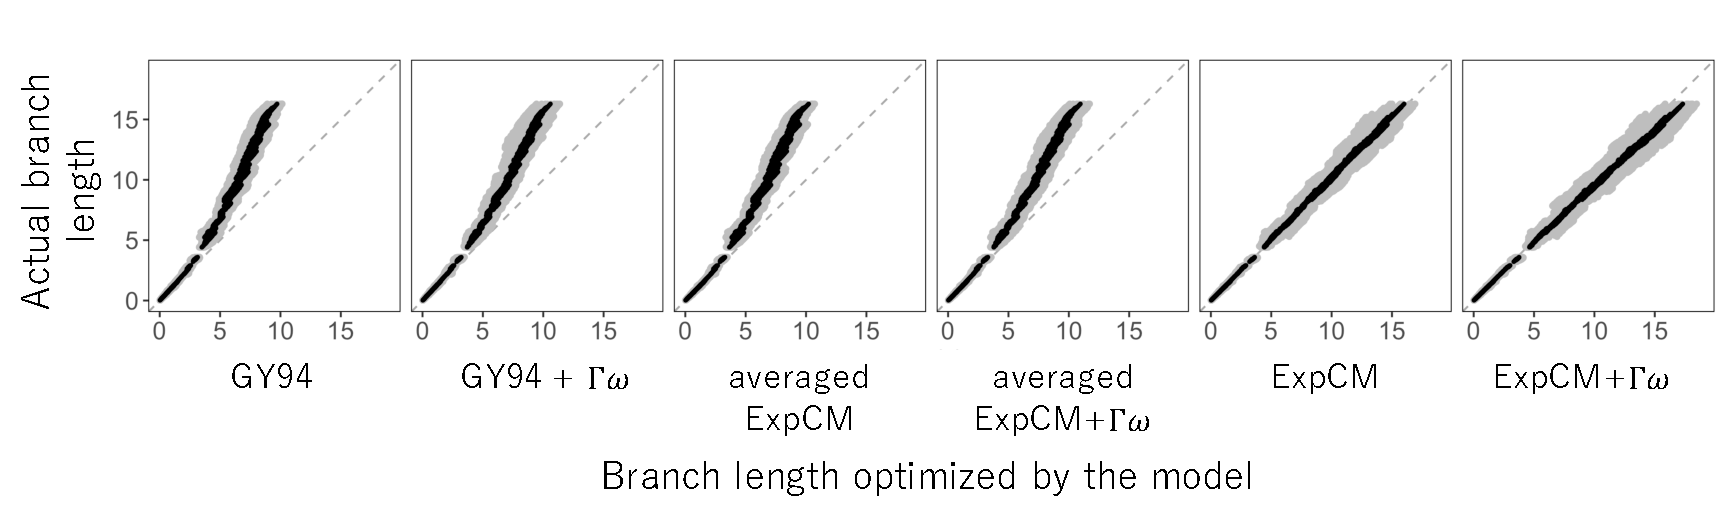
\includegraphics[width=0.85\textwidth]{figures/simulations}}
\caption{\label{simulations}
\textbf{Model performance under simulated, site-specific data.} 
\jdbcomment{Fonts are small, and tick labels definitely too small. I would show averaged.}
Alignments were simulated under an ExpCM (\ref{tab:sim_params}) along an HA tree and the branches were re-optimized by a model from the ExpCM or YNGKP family. 
The randomized ExpCMs have amino-acid profiles shuffled among the sites 
These randomized models are still site-specific but the relationship between the site and the experimental data is broken. 
Grey points represent the length of one branch and the black points are the mean branch lengths over eight simulations. 
The grey, dashed line is the reference line $y=x$, depicting the behavior of a model which is an unbiased estimator of the simulated branch length. 
}
\end{figure}

Next, we explored how accurately these models infer branch length when site-specificity is assumed, as expected in natural sequences.  
We simulated sequences under an ExpCM defined by the amino-acid preferences measured by \cite{doud2016accurate} along an influenza tree. 
We then re-inferred the branch lengths using the models described in \ref{fig:model_feature}. 

The two models with uniform stationary states, GY94 and GY94+$\Gamma\omega$, both underestimate long branches (> ~5 codon substitutions per site). 
The degree of underestimation becomes more pronounced as the branch length increases, as shown by the curve of the correlation. 
The addition of $\Gamma\omega$ rate variation does not mitigate the effect as both models show roughly the same degree of underestimation. 

Conversely, the ExpCM and ExpCM+$\Gamma\omega$ both avoid the underestimation bias, even at the longest branch lengths measured. 
As the branch length increases, the variance of the branch length estimation also increases (grey points). 
But, unlike the GY94 and the GY94+$\Gamma\omega$, the variance is unbiased in regards to under- or overestimation of the true branch length. 

Finally, the randomized control ExpCM and ExpCM+$\Gamma\omega$ show that the importance is truly in site-\textit{specificity}. 
If the preferences are randomized along sites in the protein, the model exhibits the same degree of underestimation as the GY94 and GY+$\Gamma\omega$ models. 
This underscores the point that the non-uniform stationary state models are site-specific and that mismatches are just as much of a problem as not accounting for these differences at all. 

Overall, the simulations show that if site-specificity is true, the addition of $\Gamma\omega$ will still have problems at extremely long branches. 

\subsection*{empirical Data}

Next we compared the branch lengths inferred by the different models on empirical data. 
We looked at the influenza virus surface protein hemagglutinin (HA). 
HA proteins cluster into tight phylogenetic groups with long branches in between them. 
Furthermore, HAs are extremely diverse. 
The HAs which commonly circulate in human viruses (H1 and H3) are only about 40\% identical on the amino acid level. 

\begin{figure}[H]
\centerline{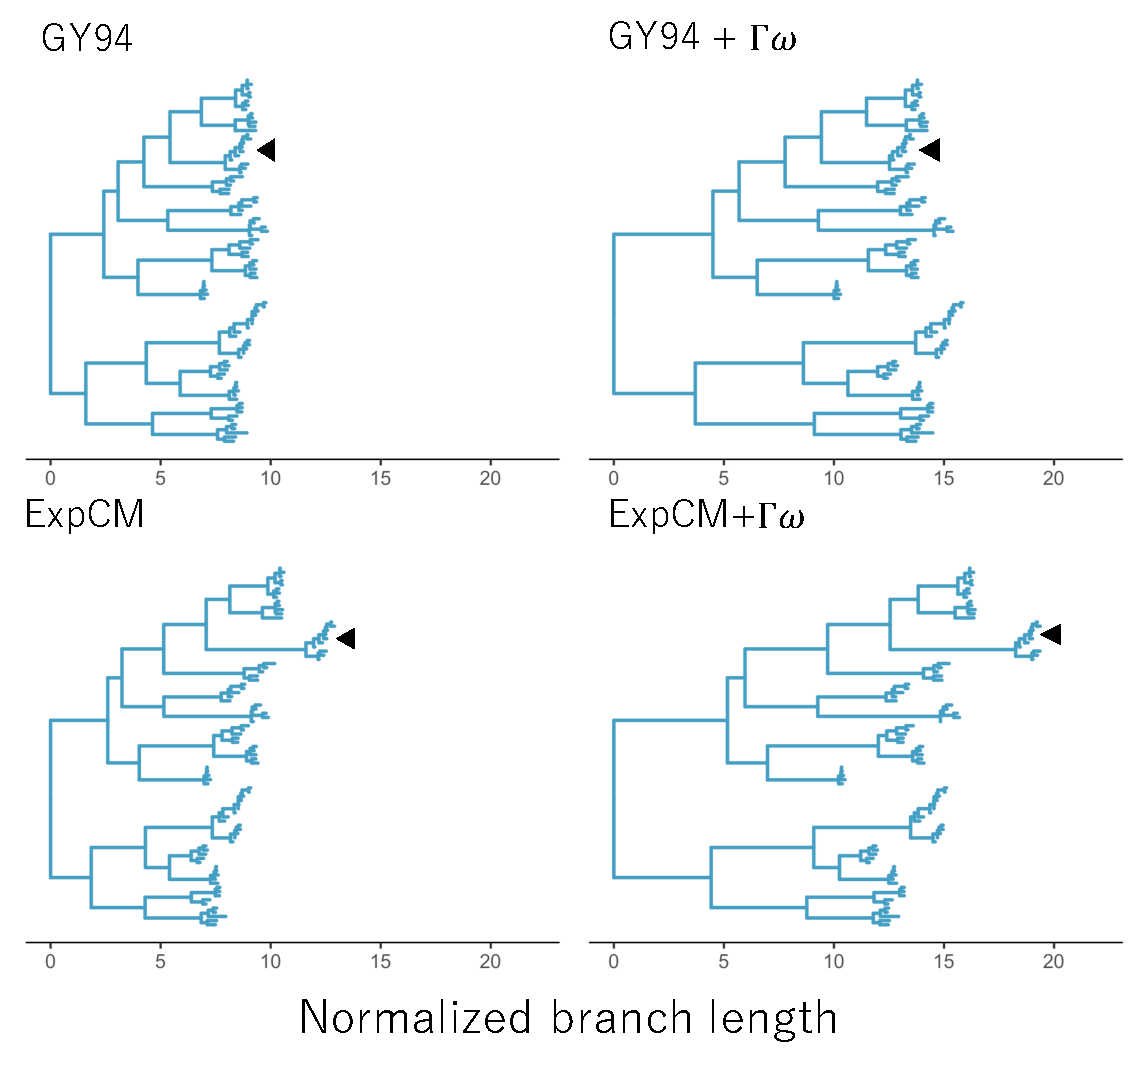
\includegraphics[width=0.5\textwidth]{figures/tree_doud}}
\caption{\label{fig:tree_doud}
\textbf{Trees optimized with an ExpCM defined by H1 preferences lengthen branches from the focal H1 sequence compared to YNGKP models.} 
\jdbcomment{Keep branch lengths in substitutions per site. Make a panel A show a prefs snippet, B H1 trees, C H3 trees, D H1+H3. Maybe increase very small font sizes a bit.}
The branch lengths of a base topology inferred using the GTR-CAT model were optimized by \textbf{(A)} an ExpCM defined by H1 preferences, \textbf{(B)} an ExpCM+$\Gamma\omega$ defined by H1 preferences, \textbf{(C)} YNKGP M0, and \textbf{(D)} YNGKP M5.
The branch lengths are normalized to the distance between A/South Carolina/1/1918 and A/Solomon Islands/3/2006 and colored to indicate the distance from the H1 focal sequence (black triangle).
}
\end{figure}

We took a representative sample of HA from 14 of the 18 groups and optimized the branch lengths of the tree using the models described in \ref{fig:model_feature}. 
First, we used an ExpCM defined by the site-specific amino-acid preferences measured by deep mutational scanning from \cite{doud2016accurate}. 
These amino-acid preferences were measured in the genetic background of the H1 strain A/Wilson-Smith/1993. 
We designate this strain (and more broadly the H1 subtype) as the focal sequence of the model. 

\ref{fig:tree_doud} shows the results. 
Comparing GY94 to GY94+$\Gamma\omega$ or ExpCM to ExpCM+$\Gamma\omega$ shows the addition of $\Gamma\omega$ causes branch length extension independent of the presence of preferences. 
In addition, comparing comparing GY94 to ExpCM or GY94+$\Gamma\omega$ to ExpCM+$\Gamma\omega$ shows that the addition of preferences causes branch length extension from the \textit{focal} sequence independent of the presence of $\Gamma\omega$. 
Together this suggests that site-specificity of the model is important because branch lengths are shorter in the absence of preferences. 
However, the preferences used here to define the ExpCM are clearly not equally relevant across all parts of the tree. 
Specifically, they are most relevant near the strain that they were measured in. 
This not at all unexpected because epistasis, where the effect of a mutation at one site is dependent on the identity of another site is well documented. 
It would surprising if epistasis \textit{was not} a factor at these large divergences across the HA tree. 

This becomes even more apparent when the performance of the ExpCM defined by H1 preferences is compared to the ExpCM with H3 preferences. 
Namely, the exact same pattern is observed. 
There is extension across the whole tree when $\Gamma\omega$ is added to the model, independent of whether or not preferences are included in the model, and there is an extension of branch lengths from the focal sequence when preferences are added, independent of whether or not $\Gamma\omega$ is included in the model. 
Finally, we defined an ExpCM with the average of the H1 and H3 preferences, which can be seen as a rough proxy for the model sampling both preference sets. 
In this model, there is an extension in branch length from \textit{both} focal sequences. 

These three sets of trees imply that site-specificity is important and not constant. 
This observation is not surprising. 
Epistasis, where the effect of a mutation at a site is dependent on the identity of another site in the protein, is well documented. 
It is not all together surprising that there are epistatic interactions between H1 and H3 due to the large sequence divergence between the two strains. 
In contrast, the deep mutational scanning preferences are measured in a single genetic background and therefore only measure the effect of mutations in one, specific genetic context.  
The difference between the trees using the H1 preferences and the H3 preferences is most likely that the preferences "shifted" due to the genetic context. 
The model with the average preferences could be seen as a proxy for a model which is able to sample both preference sets. 

\subsection{Competing effects of shifting preferences and long branches.}
We explored these competing effects of shifting preferences and long branches by comparing the effects of the model across trees which vary in overall divergence levels. 
We used the $\beta$ parameter of the ExpCM model as a proxy for the degree to which the preferences have shifted. 
In each run of the model, the parameter $\beta$ is fit and effectively rescales the preferences. 
When $\beta = 1$, we infer that selection in nature and selection in the lab prefers the same amino acids and with the same level of stringency. 
When $\beta > 1$, we infer that selection in nature prefers the same amino acids as selection in lab but with much higher stringency and when $\beta < 1$ we infer that selection in lab and selection in nature prefer different amino acids or at a \textit{much} lower stringency. 
An alternative way of saying this is that the value of $\beta$ and the perceived "relevance" of the preferences are inversely correlated. 

For each preference set, we took a subset the full HA tree shown in \ref{fig:tree_doud} or \ref{fig:tree_lee} to create a tree with either low divergence from the focal sequence (low) or intermediate divergence from the focal sequence (intermediate) and estimated the branch lengths on these trees using the same models as above. 
As we hypothesized above, as the overall divergence of the tree increases the $\beta$ value decreases. 
That is as the tree begins to include more and more sequences which are highly diverged from the focal sequence, the less relevant the preferences appear to be overall. 
As divergence increases the relevance of the preferences decreases. 

On the other hand, the effect of having a site-specific stationary state is more apparent when there are long branches on the tree.
There is no real bias in estimation in any of the models for the low or intermediate trees. 
This is not surprising as \ref{fig:decay} shows that the differences in these models really only matters at the long branches. 
The underestimation is only apparent for the "high divergence" alignment (aka the full tree). 
Here it becomes clear that you have these competing effects. 
It is most important to have the site-specificity at these long branches but it is also where the site-specific preferences are the least relevant. 


For set of preferences, 
\section*{Conclusion}

\begin{enumerate}
  \item We don't allow any of the models to vary by lineage. 
\end{enumerate}

\newpage
\section*{Materials and Methods}

\subsection*{Substitution models}
\subsubsection*{GY94 models}
\subsubsection*{ExpCMs}
We recap the \textbf{Exp}erimentally Informed \textbf{C}odon \textbf{M}odel (ExpCM) \citep{bloom2014experimentally,bloom2014informed,bloom2017identification,hilton2017phydms} to introduce nomenclature. 

In an ExpCM, rate of substitution $P_{r,xy}$ of site $r$ from codon $x$ to $y$ is written in mutation-selection form~\citep{halpern1998evolutionary,mccandlish2014modeling,spielman2015relationship} as
\begin{equation}
P_{r,xy} = Q_{xy} \times F_{r,xy}
\end{equation}
where $Q_{xy}$ is proportional to the rate of mutation from $x$ to $y$, and $F_{r,xy}$ is proportional to the probability that this mutation fixes.
The rate of mutation $Q_{xy}$ is assumed to be uniform across sites, and takes an HKY85-like~\citep{hasegawa1985dating} form:
\begin{equation}
Q_{xy} = 
\begin{cases}
\phi_w & \mbox{if $x$ and $y$ differ by a transversion to nucleotide $w$} \\
\kappa \phi_w & \mbox{if $x$ and $y$ differ by a transition to nucleotide $w$} \\
0 & \mbox{if $x$ and $y$ differ by $>1$ nucleotide.}
\end{cases}
\end{equation}
The $\kappa$ parameter represents the transition-transversion ratio, and the $\phi_w$ values give the expected frequency of nucleotide $w$ in the absence of selection on amino-acid substitutions, and are constrained by $1 = \sum_w \phi_w$.

The deep mutational scanning data are incorporated into the ExpCM via the $F_{r,xy}$ terms.
The experiments measure the preference $\pi_{r,a}$ of every site $r$ for every amino-acid $a$.
The $F_{r,xy}$ terms are defined in terms of these experimentally measured amino-acid preferences as
\begin{equation}
\label{eq:Frxy}
F_{r,xy} = 
\begin{cases}
   1 & \mbox{if $\mathcal{A}\left(x\right) = \mathcal{A}\left(y\right)$} \\
   \omega \times \frac{\ln\left[\left(\pi_{r,\mathcal{A}\left(y\right)} / \pi_{r,\mathcal{A}\left(x\right)}\right)^{\beta}\right]}{1 - \left(\pi_{r,\mathcal{A}\left(x\right)} / \pi_{r,\mathcal{A}\left(y\right)}\right)^{\beta}} & \mbox{if $\mathcal{A}\left(x\right) \ne \mathcal{A}\left(y\right)$}
   \end{cases}
\end{equation}
where $\mathcal{A}\left(x\right)$ is the amino-acid encoded by codon $x$, $\beta$ is the stringency parameter, and $\omega$ is the relative rate of nonsynonymous to synonymous substitutions after accounting for the amino-acid preferences.
The ExpCM has six free parameters (three $\phi_w$ values, $\kappa$, $\beta$, and $\omega$).
The preferences $\pi_{r,a}$ are \emph{not} free parameters since they are determined by an experiment independent of the sequence alignment being analyzed.

The ExpCM stationary state frequency $p_{r,x}$ of codon $x$ at site $r$ is~\citep{bloom2017identification} 
\begin{equation}
\label{eq:p_rx}
p_{r,x} = \frac{\left(\pi_{r,\mathcal{A}\left(x\right)}\right)^{\beta} \phi_{x_0} \phi_{x_1} \phi_{x_2}}{\sum_z \left(\pi_{r,\mathcal{A}\left(z\right)}\right)^{\beta} \phi_{z_0} \phi_{z_1} \phi_{z_2}},
\end{equation}
\subsection*{Theoretical effect of model choice on branch length}
\subsection*{Effect of model choice on natural sequences}

\subsubsection*{ExpCM + $\Gamma\omega$ and YNGKP M5}


\subsubsection*{Spielman $\omega_{r}$ values inferred from the ExpCM} 
We inferred the average nonsynonymous fixation rate from the ExpCM following~\citet{spielman2015relationship} as 
\begin{equation}
\label{eq:w_r}
\omega_{r} = \frac{\sum_{x} \sum_{y \in N_x} {p_{r,x} \times P_{r,xy}}}{\sum_{x} \sum_{y \in N_x} {p_{r,x} \times Q_{xy}}}
\end{equation}
where $p_{r,x}$ is the stationary state of the ExpCM at site $r$ and codon $x$, $P_{r,xy}$ is the substitution rate from codon $x$ to codon $y$ at site $r$, $Q_{xy}$ is the mutation rate from codon $x$ to codon $y$, and $N_x$ is the set of codons that are nonsynonymous to codon $x$ and differ from codon $x$ by only one nucleotide. 

\subsubsection*{Expected pairwise amino-acid identity}
\textit{Do I need to talk about the branchScale scaling I used?}
The expected pairwise amino-acid identity at a site $r$ over time $t$ for a given model is 
\begin{equation}
\label{eq:f}
\sum_a \sum_{x \in a} p_{r,x} \sum_{y \in a} [M_{r}\left(t\right)]_{xy}
\end{equation}
where $a$ is all amino acids, $p_{r,x}$ is the stationary state of the model at site $r$ and codon $x$, and $[M_{r}\left(t\right)]_{xy}$ is the transition rate from codon $x$ to codon $y$ at site $r$ given time $t$. 

\newpage
\section*{Supplemental Information}

\subsection*{Model Parameters for the simulations}

\begin{suppfig}[H]
\centerline{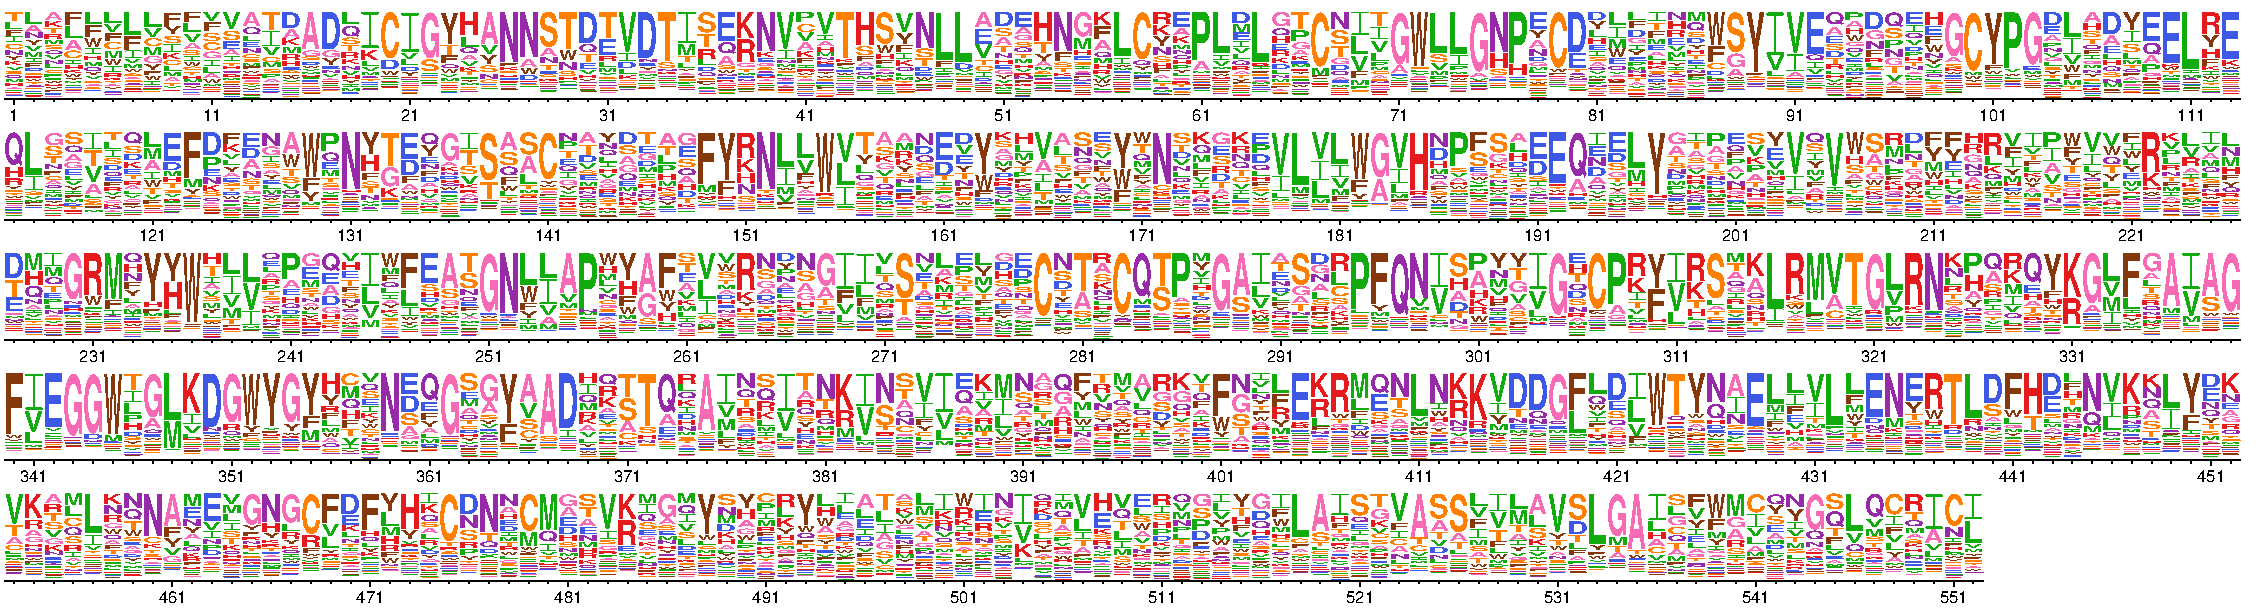
\includegraphics[width=\textwidth]{figures/prefs_doud}}
\caption{\label{suppfig:prefs_doud}
\textbf{H1 preferences measured by \cite{doud2016accurate} rescaled with the ExpCM stringency parameter optimized in \ref{fig:tree_doud}A  ($\beta = 1.21$)} 
}
\end{suppfig}

\begin{suppfig}[H]
\centerline{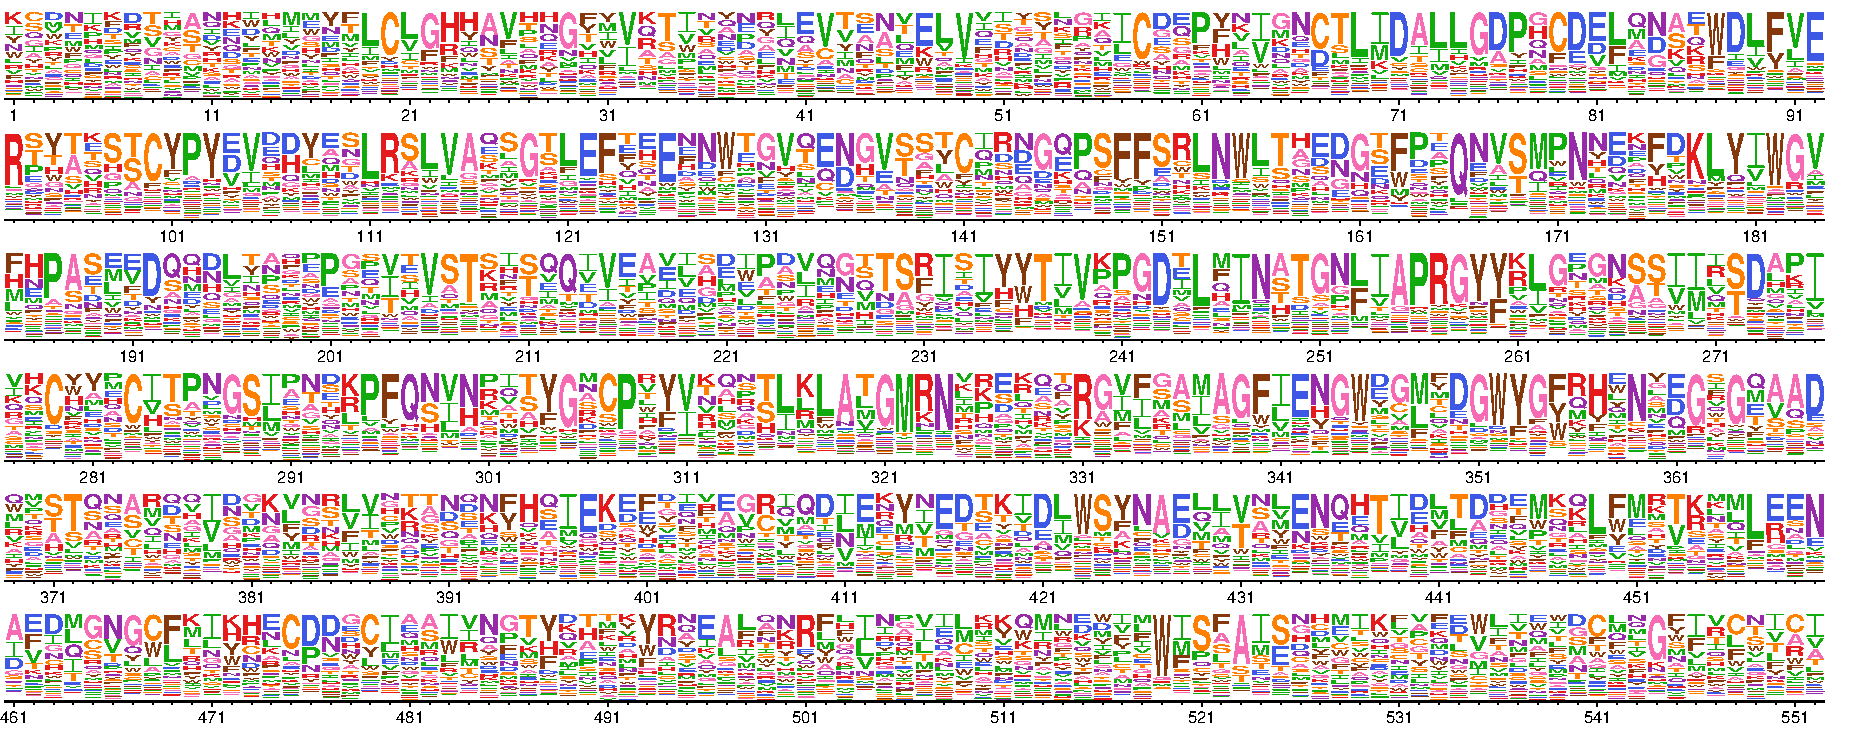
\includegraphics[width=\textwidth]{figures/prefs_lee}}
\caption{\label{suppfig:prefs_lee}
\textbf{H3 preferences measured by \textit{lee} rescaled with the ExpCM stringency parameter optimized in \ref{fig:tree_lee}A  ($\beta = 1.46$)} 
}
\end{suppfig}

\begin{figure}[H]
\centerline{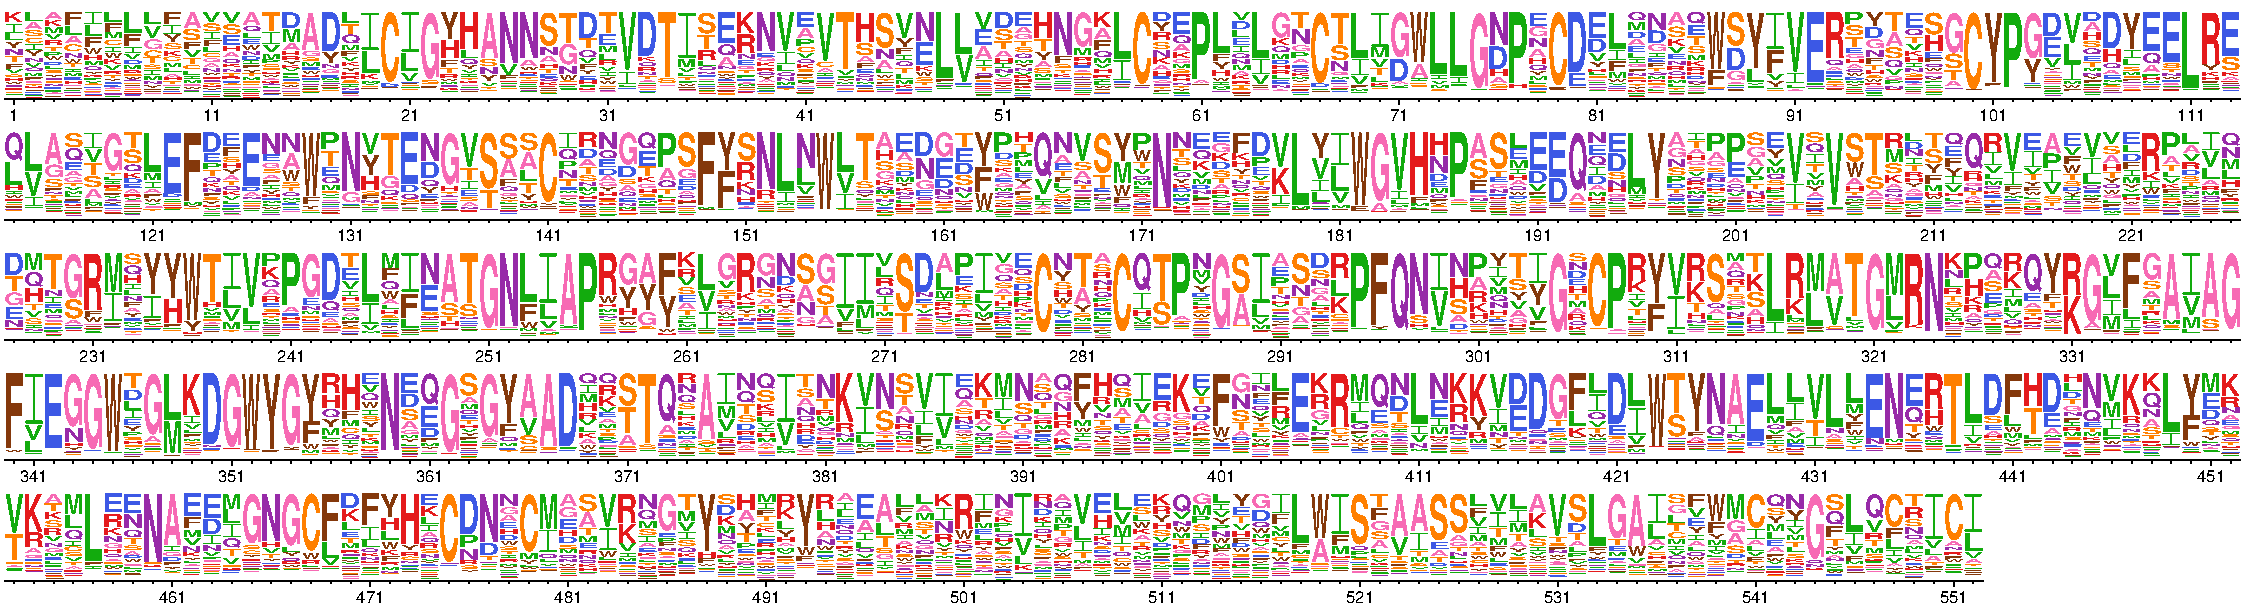
\includegraphics[width=0.85\textwidth]{figures/prefs_average}}
\caption{\label{fig:prefs_average}
\textbf{The average of the H1 preferences measured by \cite{doud2016accurate} and the H3 preferences measured by \textit{Lee} rescaled with the ExpCM stringency parameter optimized in \ref{fig:tree_average}A  ($\beta = 1.82$)}}
\end{figure}

\begin{figure}[H]
\centerline{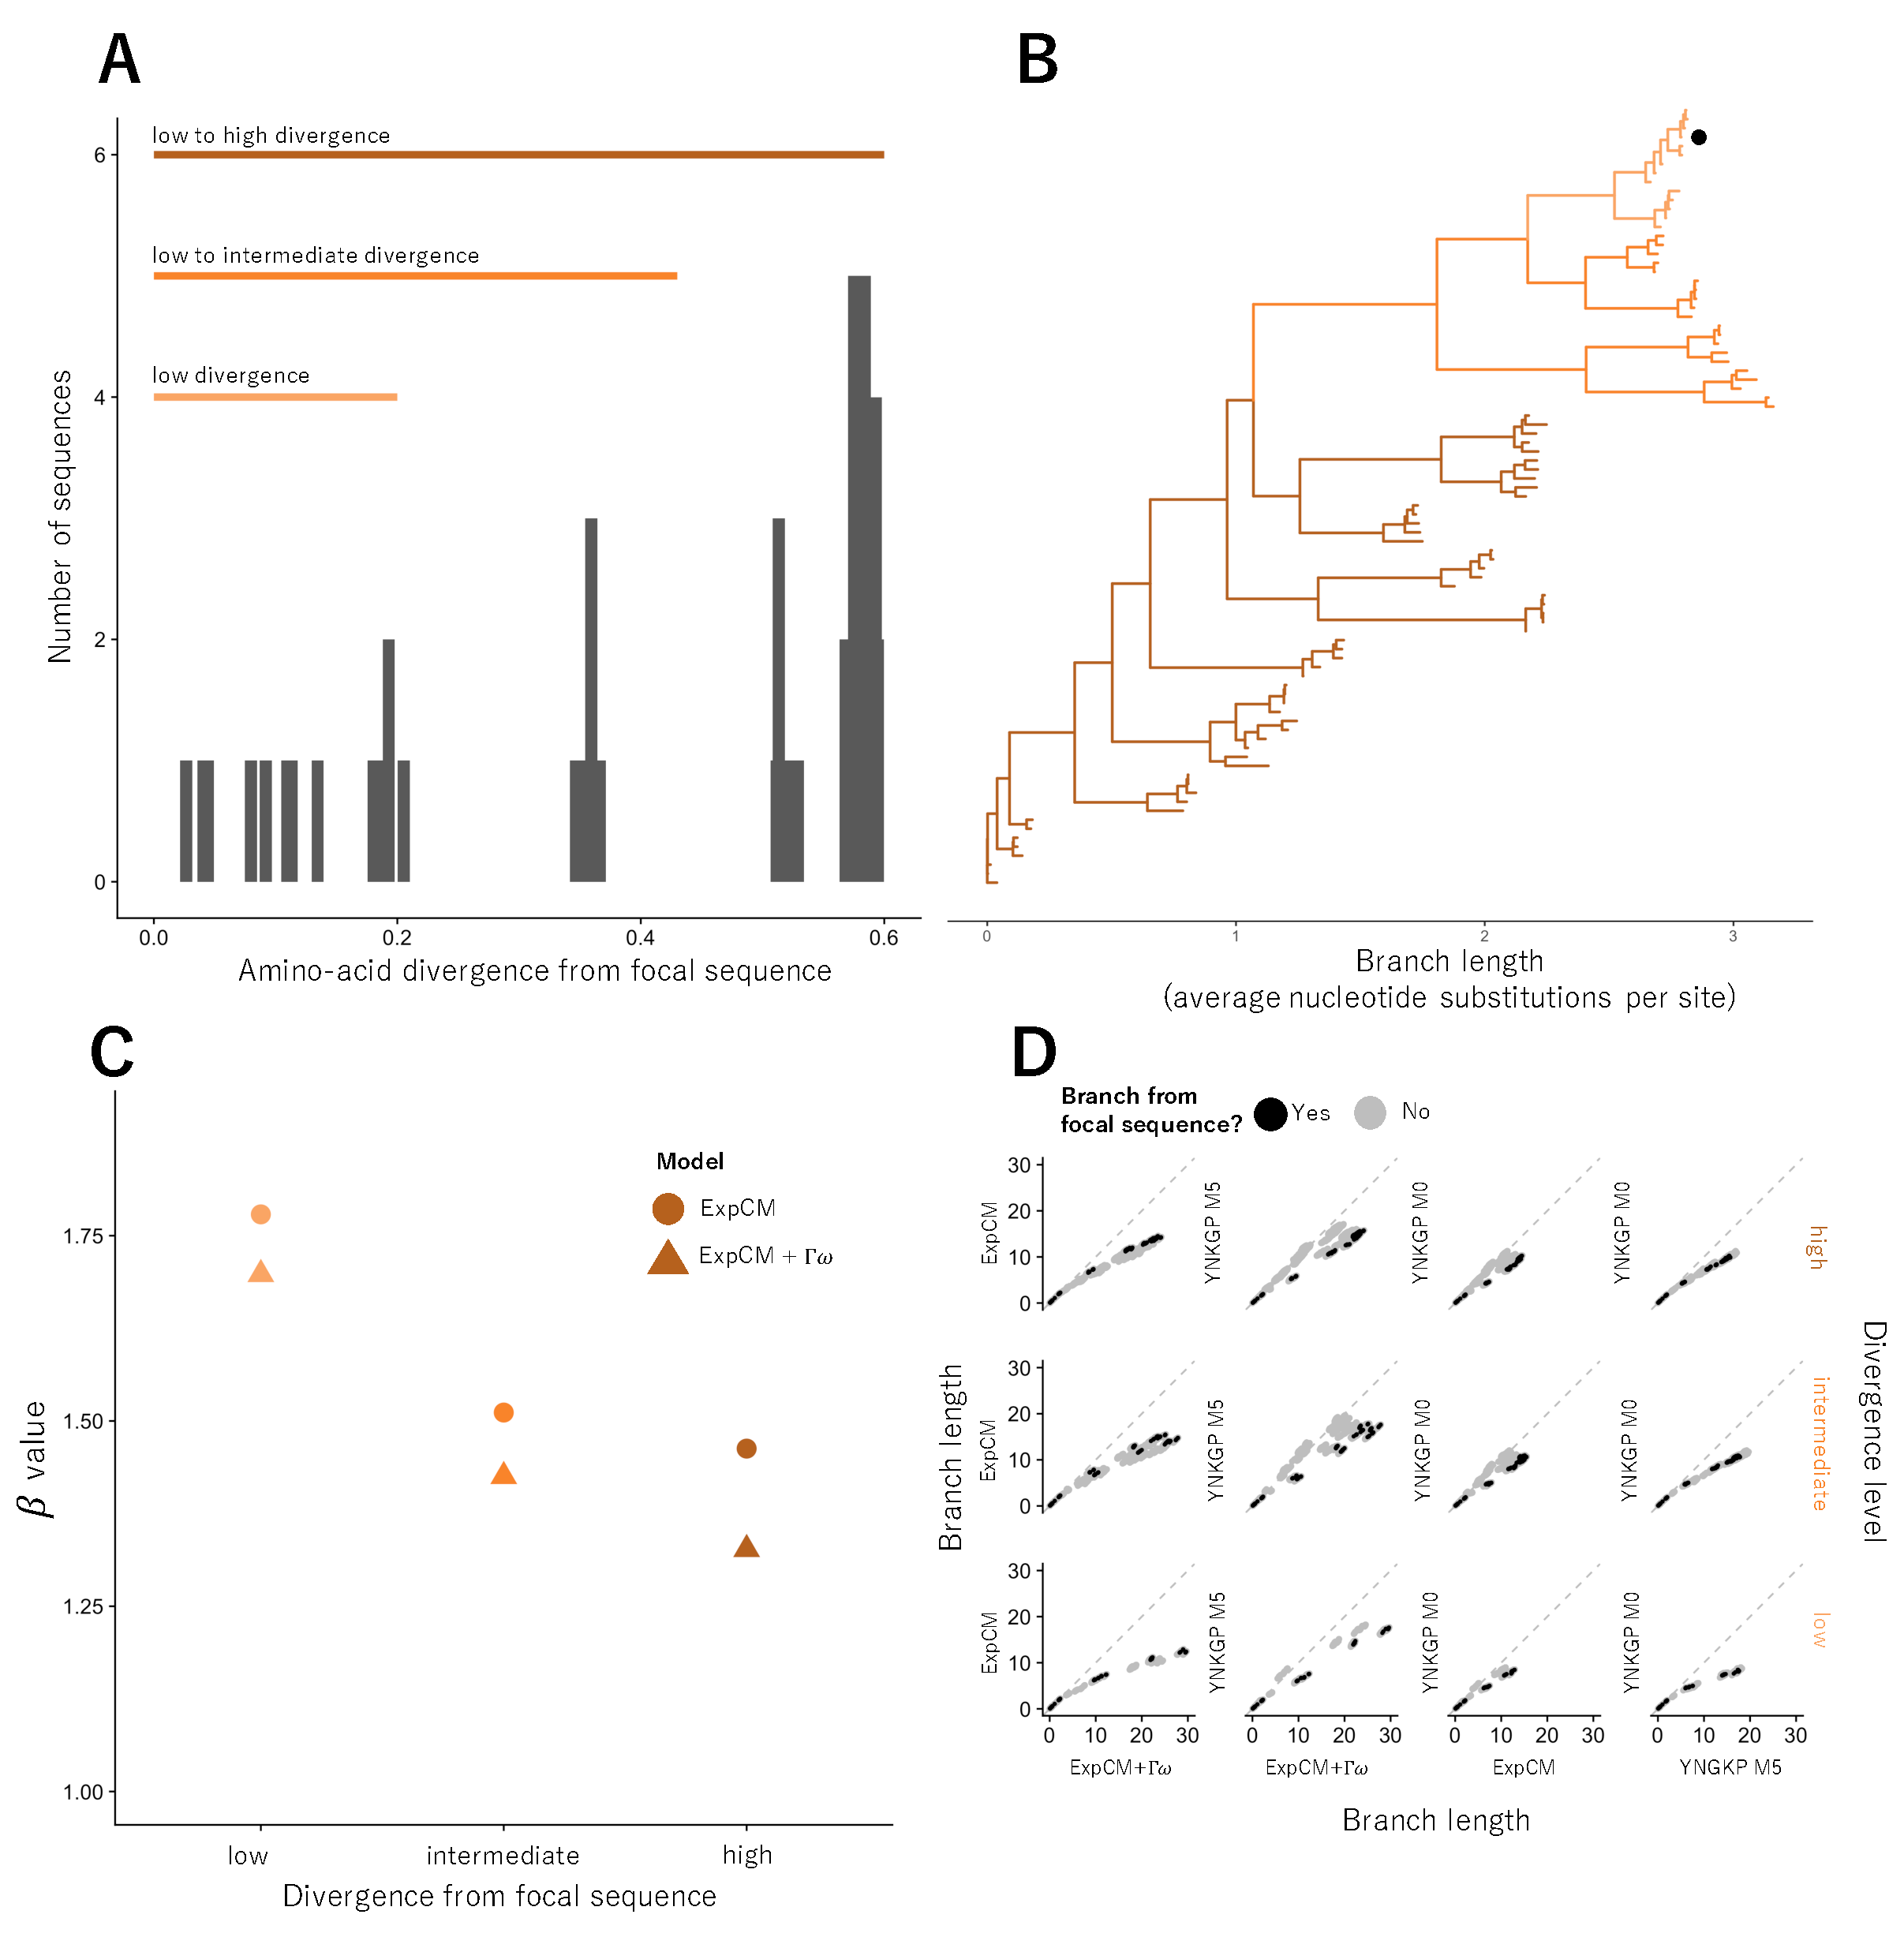
\includegraphics[width=0.85\textwidth]{figures/experiment_lee}}
\caption{\label{fig:experiment_lee}
\textbf{The ExpCM defined by H1 preferences lengthen longer branches on the HA tree.} 
\textbf{(A)} An HA alignment was subsampled to create three smaller alignments with varying degrees of divergence from the focal H3 sequence, referred to as "low", "intermediate", and "high". 
\textbf{(B)} The phylogenetic tree of the "high" alignment. 
The colors denote the alignment and the black circle denotes the focal H3 sequence. 
\textbf{(C)} The value of the ExpCM and ExpCM+$\Gamma\omega$ stringency parameter $\beta$ decreases as the divergence from the focal H3 sequence increases. 
\textbf{(D)} Comparisons of branch lengths optimized by the four substitution models for the varying degrees of divergence. 
Black points represent branches from the focal H3 sequence and grey points represent all other branches.  
The branch lengths are in average number of codon substitutions per site. 
}
\end{figure}

\begin{table}[t!]
\caption{\label{tab:simulation_params}
ExpCM parameters used to simulate sequences in Fig.~\ref{fig:simulation}.}
      \begin{tabular}{ccccc}
        \hline
          Parameter & Value\\ \hline
       	$\beta$ & $1.54$\\
	$\kappa$ & $3.60$\\
	$\omega$ & $0.20$\\
	$\phi_A$, $\phi_C$, $\phi_G$& $0.38$, $0.17$, $0.23$\\
      \end{tabular}
\end{table}

\begin{table}[t!]
\caption{\label{tab:wsn_low_params}
Model parameters used in  Fig.~\ref{fig:decay}.}
      \begin{tabular}{ccccc}
        \hline
          Model & Parameters\\ \hline
          ExpCM & $\beta=1.54196$\\
           & $\kappa=3.47184$\\
           & $\omega=0.219225$\\ 
           & $\phi_A$=0.386529\\ 
           & $\phi_C$=0.17187\\
           & $\phi_T$=0.230319\\
           & $\pi_{r, A\left(X\right)}$:Doud\\
          YNGKP M0 & $\kappa=2.9984$\\
          & $\omega=0.09076$\\
          & $\phi_{1A}=0.326007$\\
          & $\phi_{1C}=0.136307$\\ 
          &$\phi_{1G}=0.278377$\\
          &$\phi_{2A}=0.382017$\\ 
          &$\phi_{2C}=0.179763$\\ 
          &$\phi_{2G}=0.194067$\\
          &$\phi_{3A}=0.354364$\\
          &$\phi_{3C}=0.190112$\\
          &$\phi_{3G}=0.214605$\\
          YNGKP M5 & $\kappa=2.9984$\\
          & $\omega=0.09076$\\
          & $\phi_{1A}=0.326007$\\
          & $\phi_{1C}=0.136307$\\ 
          &$\phi_{1G}=0.278377$\\
          &$\phi_{2A}=0.382017$\\ 
          &$\phi_{2C}=0.179763$\\ 
          &$\phi_{2G}=0.194067$\\
          &$\phi_{3A}=0.354364$\\
          &$\phi_{3C}=0.190112$\\
          &$\phi_{3G}=0.214605$\\
      \end{tabular}
\end{table}




\begin{figure}[H]
\centerline{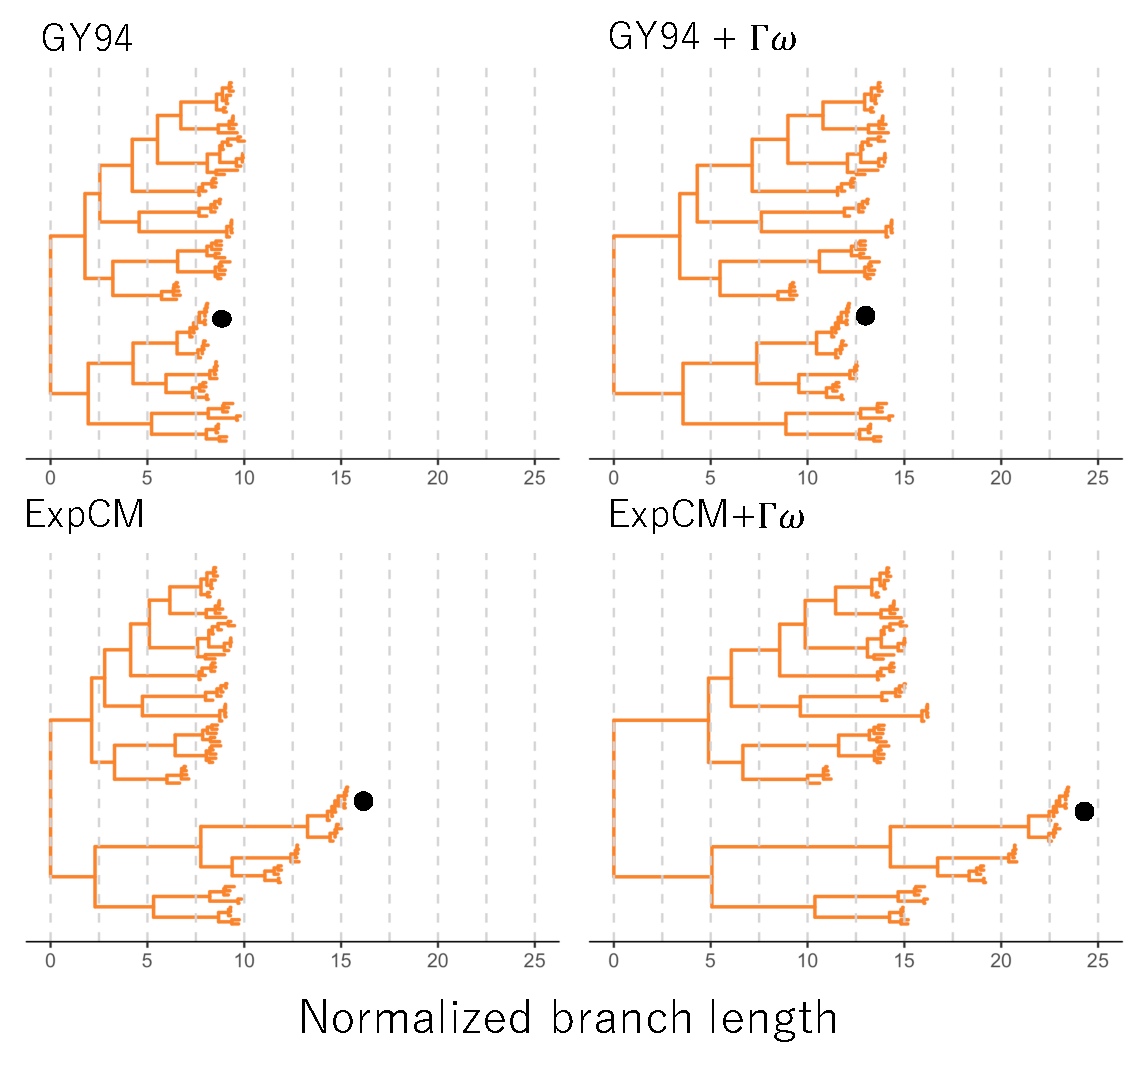
\includegraphics[width=0.85\textwidth]{figures/tree_lee}}
\caption{\label{fig:tree_lee}
\textbf{Trees optimized with an ExpCM defined by H3 preferences lengthen branches from the focal H3 sequence compared to YNGKP models.} 
The branch lengths of a base topology inferred using the GTR-CAT model were optimized by \textbf{(A)} an ExpCM defined by H3 preferences, \textbf{(B)} an ExpCM+$\Gamma\omega$ defined by H3 preferences, \textbf{(C)} YNKGP M0, and \textbf{(D)} YNGKP M5.
The branch lengths are normalized to the distance between A/South Carolina/1/1918 and A/Solomon Islands/3/2006 and colored to indicate the distance from the H3 focal sequence (black circle).
}
\end{figure}

\begin{figure}[H]
\centerline{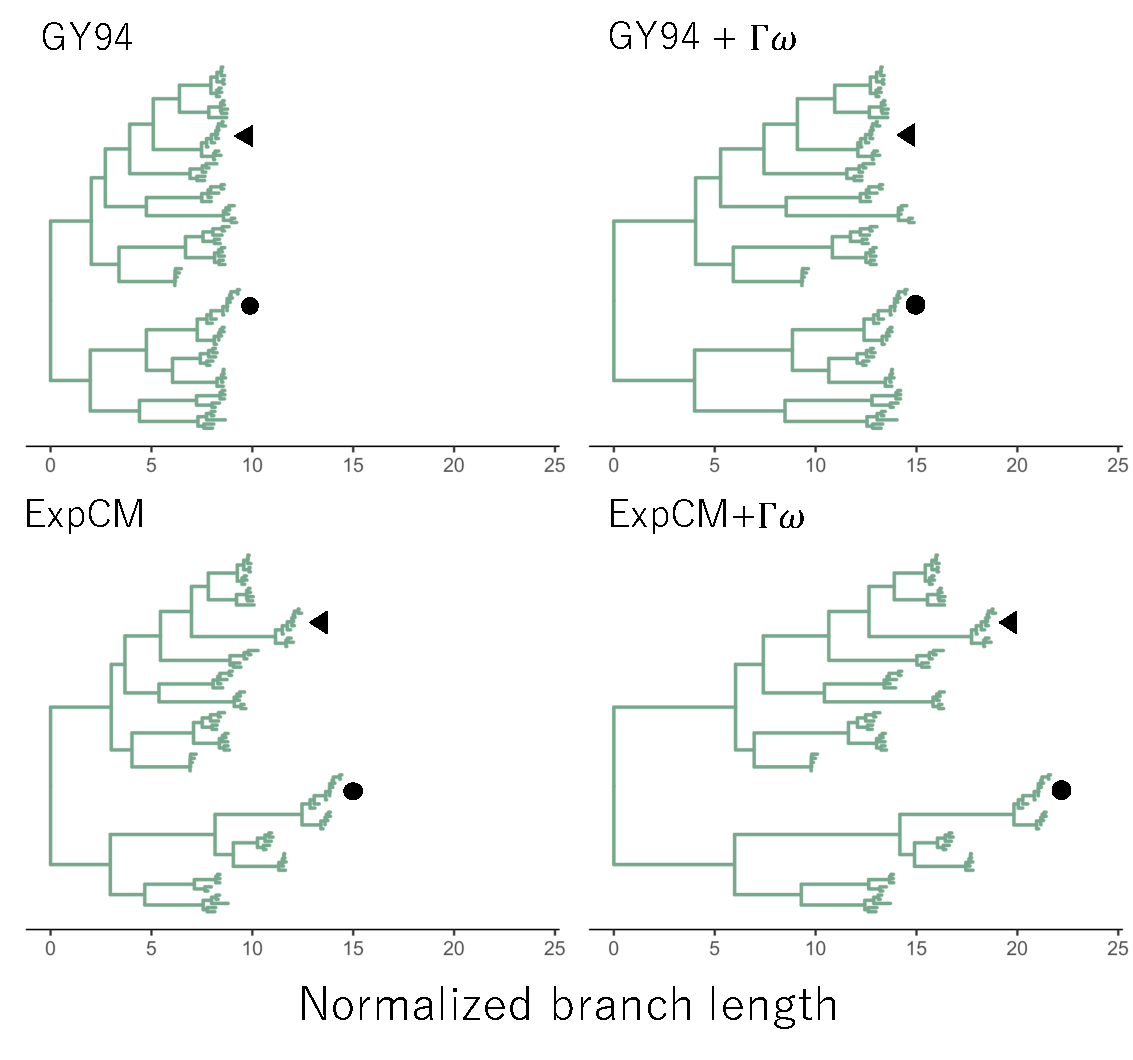
\includegraphics[width=0.85\textwidth]{figures/tree_average}}
\caption{\label{fig:tree_average}
\textbf{Trees optimized with an ExpCM defined by the average of H1 and H3 preferences lengthen branches from both the focal H3 sequence and the focal H1 sequence compared to YNGKP models.} 
The branch lengths of a base topology inferred using the GTR-CAT model were optimized by \textbf{(A)} an ExpCM defined by the average preferences, \textbf{(B)} an ExpCM+$\Gamma\omega$ defined by the average preferences, \textbf{(C)} YNKGP M0, and \textbf{(D)} YNGKP M5.
The branch lengths are normalized to the distance between A/South Carolina/1/1918 and A/Solomon Islands/3/2006.
The black triangle indicates the H1 focal sequence and the black circle indicates the focal sequence.
}
\end{figure}

\begin{figure}[H]
\centerline{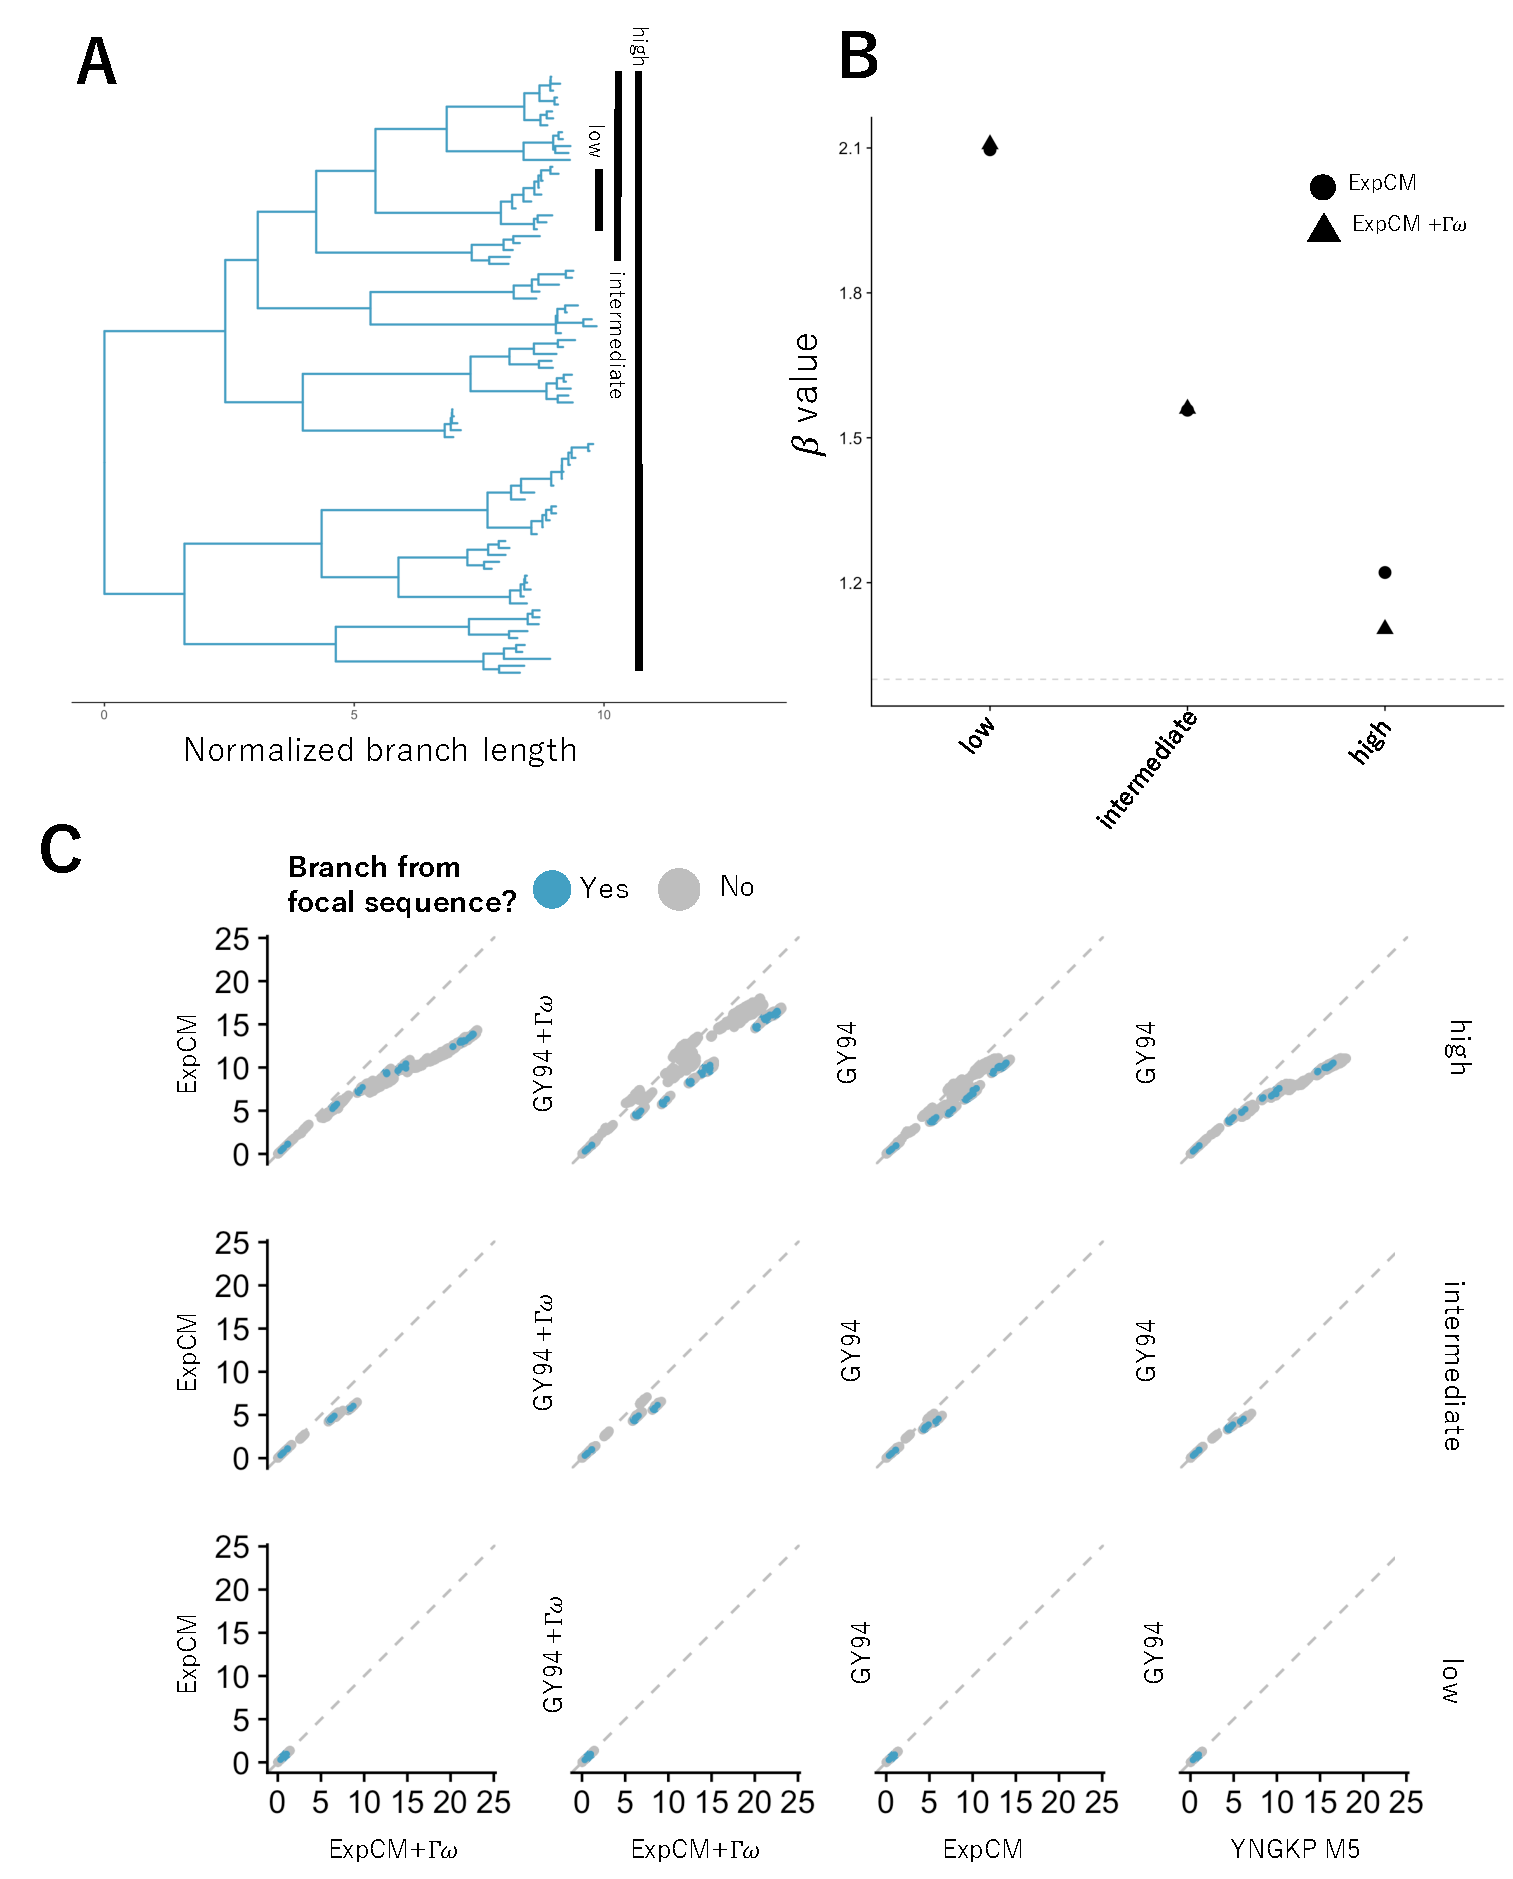
\includegraphics[width=0.85\textwidth]{figures/experiment_doud}}
\caption{\label{fig:experiment_doud}
\textbf{The ExpCM defined by H1 preferences lengthen longer branches on the HA tree.} 
\textbf{(A)} An HA alignment was subsampled to create three smaller alignments with varying degrees of divergence from the focal H1 sequence, referred to as "low", "intermediate", and "high". 
\textbf{(B)} A phylogenetic tree of the "high" alignment was constructed using the GTR-CAT model. 
The colors denote the alignment and the black circle denotes the focal H3 sequence. 
\textbf{(C)} The value of the ExpCM and ExpCM+$\Gamma\omega$ stringency parameter $\beta$ decreases as the divergence from the focal H1 sequence increases. 
\textbf{(D)} Comparisons of branch lengths optimized by the four substitution models for the varying degrees of divergence. 
Black points represent branches from the focal H3 sequence and grey points represent all other branches.  
The branch lengths are in average number of codon substitutions per site. 
}
\end{figure}

\clearpage 
\bibliographystyle{mbe}
\bibliography{references.bib}



\end{document}